\documentclass[11pt]{article}
\usepackage[margin=0.8in]{geometry}
\usepackage{bm}
\usepackage{amsfonts}
\usepackage{amsthm}
\usepackage{amssymb}
\usepackage{amsmath}
\usepackage{xcolor}
\usepackage{tikz}
\usepackage[colorlinks = true]{hyperref}

\usepackage{fancyhdr}
\pagestyle{fancy}
\fancyhf{}
\lhead{UNSW Business School}
\rhead{ACTL3182 Formula Sheet}
\cfoot{Page \thepage}  %PERHAPS Add UNSW COPYRIGHT FOOTER
\setlength{\headheight}{17pt} 

\title{\textbf{ACTL3182 Formula Sheet}}
\author{Andrew Wu}
\date{September 2020}

\usepackage{titlesec}
\titleformat{\section}{\Large\sffamily\bfseries\color{red}}{\thesection}{0.5em}{}[]
\titleformat{\subsection}{\color{red!75}\large\sffamily\bfseries}{\thesubsection}{0.5em}{}
\titleformat{\subsubsection}{\color{red!50}\normalsize\sffamily\bfseries}{\thesubsubsection}{0.5em}{}

\newcommand{\E}{\mathbb{E}}
\newcommand{\PR}{\mathbb{P}}
\newcommand{\R}{\mathbb{R}}
\newcommand{\Cov}{\operatorname{Cov}}
\newcommand{\Q}{\mathcal{Q}}

\begin{document}
	\maketitle
	\textbf{NOTE:} This is a condensed version of the cheatsheet with emphasis on formulas and little to no theory. This cheatsheet may be revised throughout the term, please check \url{https://github.com/BrownianNotion/ACTL3182_20T3.git} for the latest version.
	\section{Modern Portfolio Theory}
	\subsection{Utility Theory}
	\subsubsection{Expected Utility Theorem}
	Individual prefers \( W_1 \) over \( W_2 \) iff \( \E[U(W_1)] \geq \E[U(W_2)] \)
	\subsubsection{Investor types}
	\begin{center}
		\def\arraystretch{1.25}
	\begin{tabular}{lcccc}
		\hline
		\hline
		\textbf{Type} & \textbf{Wealth Preference} & \textbf{Utility Preference} & $\bm{U''}$ & \textbf{Concavity}\\
		\hline
		Risk-Averse & \( \E[W] \succ W \) & \( U(\E[W]) > E[U(W)] \) & \( U'' < 0 \) & concave\\
		\hline
		Risk-Neutral & \( \E[W] \sim W \) & \( U(\E[W]) = E[U(W)] \) & \( U'' = 0 \) & linear\\
		\hline
		Risk-Lover &\( \E[W] \prec W \) & \( U(\E[W]) < E[U(W)] \) & \( U'' > 0 \) & convex\\
		\hline
		\end{tabular}
	\end{center}
	\subsubsection{Risk Premium}
	The amount \( \pi(W) \) that an individual will pay to give up risk:
		\[	\pi(W) = \E[W] - c(W)\]
	where \( c(W) := U^{-1}(\E[U(W)]) \) is the \textbf{certainty wealth equivalent}.
	\subsubsection{Risk Aversion}
	Absolute risk aversion \( A(w) \) and relative risk aversion \( R(w) \)
	\[	A(w) = -\frac{U''(w)}{U'(w)},\quad R(w) = -w\frac{U''(w)}{U'(w)}.\] 
	\subsection{Investment Risk Measures}
	\subsubsection{Common Examples}
	\begin{enumerate}
		\item Variance: \( \int_{-\infty}^{\infty} (x - \mu)^2 f_{X}(x)dx \)
		\item Downside-Variance: \( \int_{-\infty}^{\mu} (x - \mu)^2 f_{X}(x)dx \)
		\item Shortfall Probability: \( \PR(X \leq L ) \)
		\item Expected Shortfall: \( \int_{-\infty}^{L}(L-x)f_{X}(x)dx \)
		\item Shortfall Variance: \( \int_{-\infty}^{L}(L-x)^2  f_{X}(x)dx \)
	\end{enumerate}
	\subsubsection{Value-at-Risk:}
	The Value-at-risk \textbf{at level }\( \bm{\alpha} \) is the maximum possible loss from holding a portfolio over a \textbf{given time period} so that the \textbf{probability of a larger loss is} \(\bm{1 - \alpha}  \).\\
	In general, 
	\[	\text{VaR}(\alpha) = \mu - X_{1 - \alpha},
		\]
	where \( X_{1-\alpha} \) is the \( 1 - \alpha \)-quantile of X.
	If \( X\sim\mathcal{N}(\mu, \sigma^2) \), then 
	\(	\text{VaR}(\alpha) = \sigma Z_{\alpha}
		\).
	\subsection{Portfolio Optimisation}
	\subsubsection{Two assets}
	Global Minimum Variance Portfolio: \[	w_A = \frac{\sigma^2_B - \sigma_{AB}}{\sigma^2_A + \sigma^2_B - 2\sigma_{AB}},\quad w_B = 1 - w_A\]
	Portfolio Variance:
	\[	\sigma_P^2 = w_A^2 \sigma_A^2 + w_B^2 \sigma_B^2 + 2w_A w_B\rho_{AB}\sigma_{A}\sigma_B\]
	
	\subsubsection{N-risky assets}
	Minimise \( \displaystyle\sigma_P^2 = \bm{w}^{\top} \Sigma \bm{w} \), \( \quad \)subject to \( \bm{1}^{\top}\bm{w}= 1 \) and \( \bm{z}^{\top}\bm{w}=\mu \).\\[5pt]
	Lagrangian: \( \mathcal{L}(\bm{w}, \lambda, \gamma)  = \frac{1}{2} \bm{w}^{\top} \Sigma \bm{w} + \lambda (1 - \bm{1}^{\top}\bm{w}) + \gamma (\mu - \bm{z}^{\top}\bm{w})\)\\\\
	Constants: \begin{align*}
				&	A = \bm{1}^{\top}\Sigma^{-1}\bm{1},\quad B =  \bm{1}^{\top}\Sigma^{-1}\bm{z} = \bm{z}^{\top}\Sigma^{-1}\bm{1}\\[2pt]
				&	C = \bm{z}^{\top}\Sigma^{-1}\bm{z}, \quad\Delta = AC - B^2\\
				\end{align*} 
	%\\[5pt]
	Minimum Variance Portfolio: 
	\[ \displaystyle\bm{w} = \lambda \Sigma^{-1} \bm{1} + \gamma \Sigma^{-1}\bm{z}  \]where \[ \lambda = \frac{C - \mu B}{\Delta}, \quad\gamma = \frac{\mu A - B}{\Delta} \]\\\\
	%\\[5pt]
	Portfolio Variance: \[ \sigma_P^2 = \frac{A\mu^2 -2B\mu + C}{\Delta} \]\\
	Global Minimum Variance Portfolio: \[ \bm{w}_g = \frac{1}{A}\Sigma^{-1}\bm{1} \]
	
	\subsubsection{N-risky assets + risk-free}
	Minimise \( \sigma_P^2 = \bm{w}^{\top} \Sigma \bm{w} \), \( \quad \)subject to \( (\bm{z} - r_{f}\bm{1})^{\top}\bm{w} = u - r_f \).\\[5pt]
	Lagrangian: \( \mathcal{L}(\bm{w}, \lambda, \gamma)  = \frac{1}{2}\bm{w}^{\top}\Sigma\bm{w} + \gamma(\mu - r_f - (\bm{z} - r_f \bm{1})^{\top}\bm{w}) \)\\\\
	Minimum Variance Portfolio: \[ \bm{w} = \gamma\Sigma^{-1}(\bm{z} - r_f \bm{1}) \] where \[ \gamma = \frac{\mu - r_f}{A r_f^2 -2B r_f + C} \]\\\\
	Portfolio Variance: \[ \sigma_P^2 = \frac{(\mu - r_f)^2}{A r_f^2 -2B r_f + C} \]\\\\
	Tangency Portfolio: \[ \bm{w}_t = \gamma_t \Sigma^{-1}(\bm{z} - r_f \bm{1}) \] where \[ \gamma_t = \frac{1}{B - Ar_f} \]

	%%%%%%%%%%%%%%%%%%%%%%%%%%%%%%%%%%%%%%%%%%%%%%%%%%%%%%%%%%%%%%%%%%%%%%%%%%%%%%%%%%%%%%%%%%
	\section{Asset Pricing Models}
	For all parts in section 2, \( i \) takes values \( 1,2,... N \) and indexes the assets in the market.
	\subsection{CAPM}
	
	\subsubsection{Capital Market Line}
	%The line representing all efficient portfolios when there are \( N \)-risky assets and a risk-free asset.
	\[	u_{e} = r_{f} + \frac{\sigma_{e}}{\sigma_{M}}(\mu_{M} - r_{f})\]
	%where \( {}_{e}, {}_{M} \) denote the efficient and Market Portfolios respectively.
	\subsubsection{Security Market Line}
	
	\begin{align*}
	&\mu_i = r_f + \beta_i (\mu_M - r_f), \quad\text{where} \\[4pt]
	&\beta_i = \frac{\sigma_{i, M}}{\sigma_{M}^2}
	\end{align*}	
	\subsubsection{Risk Decomposition}
	\begin{align*}
		\sigma_i^2 & = \beta_i^2 \sigma_M^2 + \sigma_{\xi_{i}}^2 \\
		& = \text{Systematic Risk} + \text{Non-systematic Risk}
	\end{align*}	
	\subsection{Factor Models}
	\subsubsection{Single Factor Model (SFM)}
	\[	r_i = \alpha_i + \beta_i f + \epsilon_i, \]
	where \( \alpha_i, \beta_i \) are stock-specific constants, \( f \) is the factor capturing market-wide price movement and \( \epsilon_i \) is a noise term reflecting firm-specific risk.
	\subsubsection{SFM Assumptions}
	\subsubsection{Risk Decomposition and Covariance}
	\begin{align*}
	& \sigma_i^2 = \beta_i^2 \sigma_f^2 + \sigma_{\epsilon_{i}}^2 = \text{Systematic Risk} + \text{Non-systematic Risk}\\
	& \sigma_{i, j} = \beta_i \beta_j \sigma_f^2
	\end{align*}
	\subsubsection{Diversification}	
	\[	R_P^2 = \frac{\beta_P^2 \sigma_f^2}{\sigma_P^2} = \frac{\text{Systematic Risk}}{\text{Total Risk}}\]
	Full diversification when \( R_P^2 = 1 \).
	\subsubsection{Multi-Factor Models}
	\[	r_i = \alpha_i + \beta_{i, 1}f_1 + \beta_{i, 2}f_2 + ... + \beta_{i, K} f_K + \epsilon_i \]
	Factors \( f_i \) may include inflation, economic growth, interest rates etc.
	\subsection{APT}
	\subsubsection{Single-Factor APT Returns}
	\begin{align*}
		& r_i = a_i + b_i f + \epsilon_i\\[5pt]
		& \E[r_i] = a_i,\quad \sigma_i^2 = b_i^2 + \sigma_{\epsilon_i}^2,\quad\sigma_{i, j} = b_{i}b_{j}
	\end{align*}
	Under no-arbitrage, 
	\[	a_i = \lambda_0 + \lambda_1 b_i,\]
	where \( \lambda_0 = r_f \) if there is a risk-free asset.
	\subsubsection{Multi-Factor APT Returns}
	\[	r_i = a_i + b_{i,1 }f_1 + b_{i,2} f_2 + ... + b_{i, K}f_K + \epsilon_i\]
	where
	\[	\E[r_i] = a_i = \lambda_0 + \lambda_1 b_{i,1} + \lambda_2 b_{i, 2} + ... + \lambda_K b_{i, K}\]
	and \( \lambda_0 = r_f \) if there is a risk-free asset.
	\newpage
	%%%%%%%%%%%%%%%%%%%%%%%%%%%%%%%%%%%%%%%%%%%%%%%%%%%%%%%%%%%%%%%%%%%%%%%%%%%%%%%%%%%%%%%%%
	\section{Discrete Time Derivative Pricing}
	\subsection{Options}
	Let: \( S_t \) denote the time \( t \) stock price, \( c_t, p_t \) denote the time \( t \) European call/put prices, \( T \) denote the option's maturity, \( K \) denote its strike price and \( r \) denote the risk-free rate.
	\subsubsection{Vanilla Options}
	\begin{center}
		\begin{tabular}{ccc}
			\hline
			\hline
			\textbf{Moneyness} & \textbf{European Call} & \textbf{European Put} \\
			\hline
			In the money & \( S_T > K \) & \( S_T < K \)\\
			\hline
			At the money & \( S_T = K \) & \( S_T = K \)\\
			\hline
			Out of the money &  \( S_T < K \)& \( S_T > K \)\\
			\hline
			\end{tabular}
		\end{center}
	\subsubsection{Payoff Functions and Price Bounds}
	Define \( 0\leq U\leq T \) as the exercise time for an American option. \( U:=\infty \) if option not exercised. \\Note: \( (X)_{+} := \max\{0, X\} \). Option bounds are for option prices at \textbf{time} \( \bm{t} \).
	\begin{center}
		\def\arraystretch{1.25}
		\begin{tabular}{lccc}
			\hline
			\hline
			\textbf{Option} & \textbf{Payoff} & \textbf{Lower Bound} & \textbf{Upper Bound} \\
			\hline
			European Call & \( (S_T - K)_{+} \) & \( S_t - Ke^{-r(T - t)} \) & \( S_t \)\\
			\hline
			European Put & \( (K - S_T)_{+} \) & \( Ke^{-r(T - t)} - S_t \) & \( Ke^{-r(T - t)} \) \\
			\hline
			American Call & \( (S_U - K)_{+} \) & \( S_t - Ke^{-r(T - t)} \) & \( S_t \)\\
			\hline
			American Put & \( (K - S_U)_{+} \) & \( K - S_t \) & \( K \)\\
			\hline
			\end{tabular}
		\end{center}
	\subsubsection{Position Diagrams}
	Long position = buy, short position = sell. 
	\begin{center}
		\resizebox{0.4\linewidth}{5cm}{
			\begin{tikzpicture}[baseline={(0,0)}]
			\tikzstyle{every node}=[font=\tiny];
			
			%Axes
			\draw[-latex] (0, 0) -- (3, 0) ;
			\draw[-latex] (0, -1.5) -- (0, 2);
			\node[above] at (0, 2) {\( \$ \)};
			\node[right] at (3, 0) {\( S_T \)};
			
			%Payoff curve
			\draw[red, semithick, -] (0, 0) -- (1, 0);
			\node[below] at (1, 0) {\( K \)};
			\draw[red, semithick, -stealth] (1, 0) -- (2.5, 1.5);
			\node[red, above right] at (2.4, 1.4) {Payoff};
			
			%Profit curve
			\draw[red!50, semithick, dashed] (0, -0.7) -- (1, -0.7);
			\node[left] at (0, -0.7) {\( -c_{0} \)};
			\draw[red!50, semithick, dashed, -stealth] (1, -0.7) -- (2.5, 0.8);
			\node[red!50, above right] at (2.4, 0.7) {Profit};
			\draw[black, very thin, densely dotted] (1, 0) -- (1, -0.7);
			
			%Title
			\node[above, font = \small\bfseries] at (current bounding box.north) {Long Call};
			\end{tikzpicture}
		}
	\qquad
		\resizebox{0.4\linewidth}{5cm}{
			\begin{tikzpicture}[baseline={(0,0)}]
			\tikzstyle{every node}=[font=\tiny];
			
			%Axes
			\draw[-latex] (0, 0) -- (3, 0) ;
			\draw[-latex] (0, -1.5) -- (0, 2);
			\node[above] at (0, 2) {\( \$ \)};
			\node[right] at (3, 0) {\( S_T \)};
			
			%Payoff curve
			\draw[red, semithick, -] (0, 0) -- (1, 0);
			\node[below] at (1, 0) {\( K \)};
			\draw[red, semithick, -stealth] (1, 0) -- (2.5, -1.5);
			\node[red, right] at (2.4, -1.5) {Payoff};
			
			%Profit Curve
			\draw[red!50, semithick, dashed] (0, 0.7) -- (1, 0.7);
			\node[left] at (0, 0.7) {\( c_{0} \)};
			\draw[red!50, semithick, dashed, -stealth] (1, 0.7) -- (2.5, -0.8);
			\node[red!50, right] at (2.4, -0.8) {Profit};
			\draw[black, very thin, densely dotted] (1, 0) -- (1, 0.7);
			
			%Title
			\node[above, font = \small\bfseries] at (current bounding box.north) {Short Call};
			\end{tikzpicture}
		}
		\end{center}
	\begin{center}
		\resizebox{0.4\linewidth}{5cm} {
			\begin{tikzpicture}[baseline={(0,0)}]
				\tikzstyle{every node}=[font=\tiny];
				
				%Axes
				\draw[-latex] (0, 0) -- (3, 0) ;
				\draw[-latex] (0, -1.5) -- (0, 2);
				\node[above] at (0, 2) {\( \$ \)};
				\node[right] at (3, 0) {\( S_T \)};
				
				%Payoff 
				\draw[red, semithick, -] (0, 1) -- (1, 0);
				\node[below] at (1, 0) {\( K \)};
				\node[left] at (0, 1) {\( K \)};
				\draw[red, semithick, -stealth] (1, 0) -- (2.5, 0);
				\node[red, above] at (2.5, 0) {Payoff};
				
				%Profit
				\draw[red!50, semithick, dashed] (0, 0.3) -- (1, -0.7);
				\node[left] at (0, -0.7) {\( -p_{0} \)};
				\draw[red!50, semithick, dashed, -stealth] (1, -0.7) -- (2.5, -0.7);
				\node[red!50, below] at (2.5, -0.7) {Profit};
				\draw[black, very thin, densely dotted] (1, 0) -- (1, -0.7);
				\draw[black, very thin, densely dotted] (0, -0.7) -- (1, -0.7);
				
				%Title
				\node[above, font = \small\bfseries] at (1.6, 2.4) {Long Put};
			\end{tikzpicture}
		}
		\qquad
		\resizebox{0.4\linewidth}{5cm} {
			\begin{tikzpicture}[baseline={(0,0)}]
			\tikzstyle{every node}=[font=\tiny];
			
			%Axes
			\draw[-latex] (0, 0) -- (3, 0) ;
			\draw[-latex] (0, -1.5) -- (0, 2);
			\node[above] at (0, 2) {\( \$ \)};
			\node[right] at (3, 0) {\( S_T \)};
			
			%Payoff 
			\draw[red, semithick, -] (0, -1) -- (1, 0);
			\node[below] at (1, 0) {\( K \)};
			\node[left] at (0, -1) {\( -K \)};
			\draw[red, semithick, -stealth] (1, 0) -- (2.5, 0);
			\node[red, below] at (2.5, 0) {Payoff};
			
			%Profit
			\draw[red!50, semithick, dashed] (0, -0.3) -- (1, 0.7);
			\node[left] at (0, 0.7) {\( p_{0} \)};
			\draw[red!50, semithick, dashed, -stealth] (1,0.7) -- (2.5, 0.7);
			\node[red!50, above] at (2.5, 0.7) {Profit};
			\draw[black, very thin, densely dotted] (1, 0) -- (1, 0.7);
			\draw[black, very thin, densely dotted] (0, 0.7) -- (1, 0.7);
			
			%Title
			\node[above, font = \small\bfseries] at (current bounding box.north) {Short Put};
			\end{tikzpicture}
		}
		\end{center}
	\subsubsection{Put-Call Parity}
	Under no arbitrage, for \( 0\leq t\leq T \):
	\[	c_t + Ke^{-r(T - t)} = p_t + S_t
		\]
	\subsection{Discrete Time Pricing}
	\subsubsection{One Period Binomial Model}
	%Let \( s_u, s_d \) be the value of the stock in one period \( \delta t \) if the price goes up/down and likewise let \( f_u, f_d \) be the payoff the derivative. Let \( X \) be the payoff of the derivative at maturity.
	\begin{center}
		\resizebox{3.5cm}{4cm}{
			\begin{tikzpicture}
				%\tikzstyle{every node}=[font=\small];
				
				%Level 1
				\filldraw[fill=black] (0, 0) circle(1pt);
				\node[left] at (0, 0) {\( s_1 \)};
				
				%Lines
				\draw[-latex] (0, 0) -- (2, 1.3) ;
				\draw[-latex] (0, 0) -- (2, -1.3);
				
				%Level 2
				\node[above right] at (1.9, 1.2) {\( s_3 \)};
				\node[below right] at (1.9, -1.2) { \( s_2 \)};
				
				%Title
				\node[above, font = \small\bfseries] at (current bounding box.north) {Stock};
			\end{tikzpicture}
		}
		\hspace{2cm}
		\resizebox{3.5cm}{4cm}{
			\begin{tikzpicture}
				%\tikzstyle{every node}=[font=\small];
				
				%Level 1
				\filldraw[fill=black] (0, 0) circle(1pt);
				\node[left] at (0, 0) {\( f_1 \)};
				
				%Lines
				\draw[-latex] (0, 0) -- (2, 1.3) ;
				\draw[-latex] (0, 0) -- (2, -1.3);
				
				%Level 2
				\node[above right] at (1.9, 1.2) {\( f_3 \)};
				\node[below right] at (1.9, -1.2) { \( f_2 \)};
				
				%Title
				\node[above, font = \small\bfseries] at (current bounding box.north) {Derivative};
			\end{tikzpicture}
		}
		\end{center}
	The replicating portfolio (stocks, bonds) is:
	\[	\phi = \frac{f_3 - f_2}{s_3 - s_2},\quad \psi = \frac{1}{B(0)}e^{-r\delta t}(f_3 - \phi s_3)\]
	The derivative price today is:
	\[	V_0 = \phi s_1 + \psi B(0)
		\]
	Rewriting with risk-neutral probabilities:
	\[	V_0 = e^{-r\delta t}(q f_3 + (1 - q) f_2) = e^{-r\delta t}\E^{\Q}[X] 
		\]
	where \[ \displaystyle q = \frac{s_1 e^{r\delta t} - s_2}{s_3 - s_2}. \]
	\subsubsection{Multi-Period Binomial Model}
	Apply the one-period Binomial model to each internal node and recurse work backwards to find price.\\As an example, below is the two-period binomial model price:
	\begin{center}
		\resizebox{5cm}{5.5cm}{
			\begin{tikzpicture}
				%\tikzstyle{every node}=[font=\small];
				
				%Title
				%\node[above, font = \small\bfseries] at (current bounding box.north) {Stock};
				
				%Level 1
				\filldraw[fill=black] (0, 0) circle(2pt);
				\node[left] at (0, 0) {\( s_1 \)};
				
				%Lines
				\draw[-latex] (0, 0) -- (2, 1.5);
				\draw[-latex] (0, 0) -- (2, -1.5);
				
				%Level 2
				\node[above] at (1.9, 1.4) {\( s_3 \)};
				\node[below] at (1.9, -1.4) { \( s_2 \)};
				
				%Lines
				\draw[-latex] (2, 1.5) -- (4, 2.25);
				\draw[-latex] (2, 1.5) -- (4, 0.75);
				\draw[-latex] (2, -1.5) -- (4, -0.75);
				\draw[-latex] (2, -1.5) -- (4, -2.25);
				
				%Level 3
				\node[right] at (4, 2.25) {\( s_7 \)};
				\node[right] at (4, 0.75) {\( s_6 \)};
				\node[right] at (4, -0.75) {\( s_5 \)};
				\node[right] at (4, -2.25) {\( s_4 \)};
				
				%Title
				\node[above, font = \small\bfseries] at (current bounding box.north) {Stock};
			\end{tikzpicture}
		}
	\hspace{2cm}
		\resizebox{5cm}{5.5cm}{
			\begin{tikzpicture}
				%\tikzstyle{every node}=[font=\small];
				
				%Title
				%\node[above, font = \small\bfseries] at (current bounding box.north) {Stock};
				
				%Level 1
				\filldraw[fill=black] (0, 0) circle(2pt);
				\node[left] at (0, 0) {\( f_1 \)};
				
				%Lines
				\draw[-latex] (0, 0) -- (2, 1.5);
				\draw[-latex] (0, 0) -- (2, -1.5);
				
				%Level 2
				\node[above] at (1.9, 1.4) {\( f_3 \)};
				\node[below] at (1.9, -1.4) { \( f_2 \)};
				
				%Lines
				\draw[-latex] (2, 1.5) -- (4, 2.25);
				\draw[-latex] (2, 1.5) -- (4, 0.75);
				\draw[-latex] (2, -1.5) -- (4, -0.75);
				\draw[-latex] (2, -1.5) -- (4, -2.25);
				
				%Level 3
				\node[right] at (4, 2.25) {\( f_7 \)};
				\node[right] at (4, 0.75) {\( f_6 \)};
				\node[right] at (4, -0.75) {\( f_5 \)};
				\node[right] at (4, -2.25) {\( f_4 \)};
				
				%Risk Neutral probabilities.
				\node[red!75, above] at (1, 0.8) {\( q_1 \)};
				\node[red!75, above] at (3, -1.1) {\( q_2 \)};
				\node[red!75, above] at (3, 1.9) {\( q_3 \)};
				%Title
				\node[above, font = \small\bfseries] at (current bounding box.north) {Derivative};
			\end{tikzpicture}
		}
		\end{center}
	For \( j = 1,2,3 \):
	\[	q_j = \frac{s_{j}e^{r\delta t} - s_{2j}}{s_{2j+1} - s_{2j}}, \quad
		f_{j} = e^{-r\delta t}\left[q_{j} f_{2j+1} + (1-q_{j})f_{2j}\right]
			\]
	Substituting \( f_2, f_3 \) into \( f_1 \),
	\[	f_1 = e^{-2\delta t}\left[q_1q_3 f_7 + q_1 (1- q_3) f_6 + 
								  (1-q_1) q_2 f_5 + (1 - q_1)(1-q_2) f_4\right]
		\]

	%%%%%%%%%%%%%%%%%%%%%%%%%%%%%%%%%%%%%%%%%%%%%%%%%%%%%%%%%%%%%%%%%%%%%%%%%%%%%%%%%%%%%%%%%
	\section{Continuous Time Derivative Pricing}
	
	\subsection{Stochastic Calculus} 
	\subsubsection{Stochastic Differential Equation}
	Suppose the stochastic process \( X(t) \) can be written as
	\[	X(t) = x_0 + \int_{0}^{t} a(s) ds + \int_{0}^{t} b(s) dW(s)\]
	where \( a(\cdot), b(\cdot) \) are appropriate functions (possibly stochastic processes) and \( x_0 \) is a constant.\\
	This is abbreviated as
	\[	dX(t) = a(t) dt + b(t) dW(t), \qquad X(0) = x_0.\]
	\subsubsection{It\^{o}'s Lemma}
	Let \( f(x), F(t, x) \) be deterministic functions with continuous (partial) derivatives up to the second order. Then, 
	\begin{align*}
		& df(X(t)) = f'(X(t)) dt + \frac{1}{2}f''(X(t)) dX(t)^2 \\
		& dF(t, X(t)) = \frac{\partial F}{\partial t}dt + \frac{\partial F}{\partial x} dX(t) + \frac{1}{2}\frac{\partial^2 F}{\partial x^2} dX(t)^2
	\end{align*}
	It\^{o} multiplication table:
	\begin{center}
		\begin{tabular}{ccc}
			\( \times \) & \( dt \) & \( dW(t) \)\\
			\hline
			\hline
			\( dt \) & 0 & 0 \\
			\hline
			\( dW(t) \) & 0 & dt \\
			\hline
			\end{tabular}
		\end{center}
	\subsubsection{Girsanov-Theorem}
	Suppose \( W(t) \) is a \( \PR \)-Brownian Motion and \( \gamma(\cdot) \) is a pre-visible process. Then there exists an equivalent measure \( \Q \) with Radon-Nikodym derivative 
	\[	\zeta_t = \exp\left[-\int_{0}^{t}\gamma(s)dW(s) - \int_{0}^{t}\gamma(s)^2 ds\right]
		\]
	such that \( W^{Q} \), where
	\[	W^{\Q}(t) = W(t) - \int_{0}^{t} \gamma(s)ds,\]
	is a \( \Q \)-Brownian Motion.
	\subsection{Pricing Framework}
	\subsection{Black-Scholes-Merton Model}
	\subsubsection{Stock Process}
	The stock process follows a Geometric Brownian Motion
	\begin{align*}
	&S(t) = S_0 e^{\left(\mu - \frac{1}{2} \sigma^2\right)t + W(t)}
	%\exp\left[\left(\mu - \frac{1}{2}\sigma^2\right)t + \sigma W(t)\right]
	\\[4pt]
	\iff &dS(t) = \mu S(t) dt + \sigma S(t) dW(t)
	\end{align*}
	\subsubsection{Put and Call Formulas}
	%Consider options with underlying stock \( S(t) \), maturity \( T \) and strike price \( K \). 
	Define:
	\begin{align*}
		d_1 = \frac{\ln\left(S(t)/ K\right) +\left(r + \frac{1}{2}\sigma^2\right)(T - t)}{\sigma\sqrt{T - t}},\qquad d_2 
		%= \frac{\ln\left(S(t)/ K\right) +\left(r - \frac{1}{2}\sigma^2\right)(T - t)}{\sigma\sqrt{T - t}} 
		= d_1 - \sigma\sqrt{T - t}
	\end{align*}
	Then,
	\begin{align*}
		& c_t = S(t)N(d_1) - Ke^{-r(T - t)}N(d_2)\\[4pt]
		& p_t = Ke^{-r(T - t)}N(-d_2) - S_t N(-d_1),
	\end{align*}
	where \( N(\cdot) \) is the cdf of the standard normal distribution.
	%%%%%%%%%%%%%%%%%%%%%%%%%%%%%%%%%%%%%%%%%%%%%%%%%%%%%%%%%%%%%%%%%%%%%%%%%%%%%%%%%%%%%%%%%
	\section{Term Structure Modelling and Asset-Liability Management}
	\subsection{Short-Rate Models}
	%Merton Model: \( dr(t) = \alpha dt + \sigma dW(t) \)\\
	%Vasicek Model: \( dr(t) = \alpha (\mu - r(t)) dt + \sigma dW(t) \)\\
	%Cox-Ingersoll-Ross (CIR) Model: \( dr(t) = \alpha(\mu - r(t))dt + \sigma\sqrt{r(t)} dW(t) \)\\
	%Hull-White Model: \( dr(t) = \alpha(t)(\mu(t) - r(t))dt + \sigma(t)dW(t) \)
	\subsubsection{Merton Model:}
	\[	
		dr(t) = \alpha dt + \sigma dW(t)
			\]

	\subsubsection{Hull White Model:}
	\[	
		dr(t) = \alpha(t)(\mu(t) - r(t))dt + \sigma(t)dW(t)
		\]
	
	\subsubsection{Vasicek Model:}
	\[	dr(t) = \alpha (\mu - r(t)) dt + \sigma dW(t)
		\]

	\subsubsection{CIR Model:}
	\[	dr(t) = \alpha(\mu - r(t))dt + \sigma\sqrt{r(t)} dW(t)
		\]
	
	\subsection{Ho-Lee Model}
	\subsubsection{Definition}
	\[	r(k, s) = a(k) + b(k) s
		\]
	where \( k = \)time and \( s =  \) number of jumps. 
	\begin{align*}
		\begin{matrix}
		  	& & r(2,2)\\
			& r(1, 1) & r(2,1)\\
		r(0, 0)	& r(1, 0) & r(2,0)
		\end{matrix}
		\qquad\qquad
		\begin{matrix}
			& & a(2) + 2b(2)\\
			& a(1) + b(1) & a(2) +b(2)\\
			a(0) & a(1) & a(2)
		\end{matrix}
	\end{align*}
	\subsubsection{Calibration}
	In general,
	\[	b(k) = 2\cdot \text{st.dev}(r(k))
		\]
	The parameters \( a(k) \) are found by equating with price of Zero-Coupon Bonds. Take \( q = 1/2 \) in most situations.
	\begin{align*}
			& B(0, 1) = \frac{1}{1+a(0)}\\[3pt]
			& B(0,2) = \frac{1}{1+a(0)}\left((1 - q)\frac{1}{1 + a(1)} + q\frac{1}{1 + a(1) + b(1)}\right)
	\end{align*}
	%\subsection{Asset-Liability Management}
	\end{document}